\documentclass[12pt,a4paper,pdflatex]{disser}
\usepackage[russian]{babel}
%\usepackage[utf-8]{inputenc}
%\usepackage{amsmath,amssymb}
%\usepackage{longtable}
\usepackage{parskip}
\usepackage{caption}
\usepackage{textcomp}
\usepackage{gensymb}
\usepackage[dvips]{graphicx}
%\usepackage{wrapfig}
%\usepackage{amssymb}*
%\usepackage{color}
%\usepackage{ulem}
\usepackage{setspace}
\usepackage{hyperref}

\oddsidemargin=-0.5 cm
\evensidemargin=-0.5 cm
\textwidth=170 mm
\textheight=260 mm
\topmargin=0 cm
\voffset= -2cm
\pagenumbering{true}
%\newlength{\varheight}
%\setlength{\varheight}{3.1cm}
\setlength{\parindent}{0cm}
%\newcommand{\taskname}[name]{\begin{center} \bf{\Large{name}} \end{center}}
\spacing{1.1}
\parskip=2mm
\captionsetup[figure]{labelformat=empty}
\clubpenalty=10000
\widowpenalty=10000

\begin{document}

\begin{center}
\LARGE{Task 22}
\end{center}

\vspace{5mm}

1. The current in the strip
$$
  I=nevab,
$$
where $v$ is the velocity of electrons, $a=2$ cm is the width, $b$ is the thickness of the strip. The Hall voltage is
$$
  V=Bva=\frac{BI}{neb},
$$
which implies
$$
  b=\frac{BI}{neV}=5.30\cdot 10^{-7} \text{ m},
$$
which corresponds to green (RGB $94,255,0$)\footnote{According to \url{http://academo.org/demos/wavelength-to-colour-relationship/}}.

2. The internal difference is that the incandescent lamp is hot and the gas lamp isn't. The first one has a continuous Planck spectrum of a hot (black)body, the second one has a line spectrum of the sodium or mercury (or of whatever is inside) atoms. As it can be seen, hot lamps produce ``hot'' light which is natural and similar to the sun radiation. The cold lamps produce monochrome (sodium, mercury) or ``cold'' light (fluorescent layers) which is typically equally distributed over the visible frequency range.

3. Assuming the temperature dependence of the RTD's resistance to be $r=r_0+\alpha t$, where $t$ is the Celsius temperature. Then, as the bridge is balanced at $0\degree$C, the resistance is $r_0=25\,\Omega$. At the unknown temperature the RTD's resistance is $r=37\,\Omega$, so the temperature
$$
  t=\frac{r-r_0}{\alpha}=3057\degree \text{C}.
$$

4. If the voltage across the lead is given by $\Delta V=-S\Delta T$ with natural signs, then the change of the voltage for two leads is
$$
  \delta V=(S_1-S_2)\delta T.
$$
For a numeric calculation a value of $S$ for chrome is necessary.
\pagebreak

\begin{center}
\LARGE{Task 23}
\end{center}

\vspace{5mm}

1. The potential inside (maybe, also outside) the cylinder is given by
$$
  \phi(\rho,\varphi)=\frac{4}{\pi}\sum\limits_{m=0}^{\infty} \frac{1}{2m+1}\rho^{2m+1}\sin(2m+1)\varphi=\frac{2i}{\pi}\left(\text{arcth}\,\rho e^{-i\varphi}-\text{arcth}\,\rho e^{i\varphi}\right),
$$
where $\rho$ and $\phi$ are dimensionless (normalized) variables and $\text{arcth}\,x$ is the inverse hyperbolic tangent function. The plot of this dependence is given below.
\begin{figure}[!h]
\begin{center}
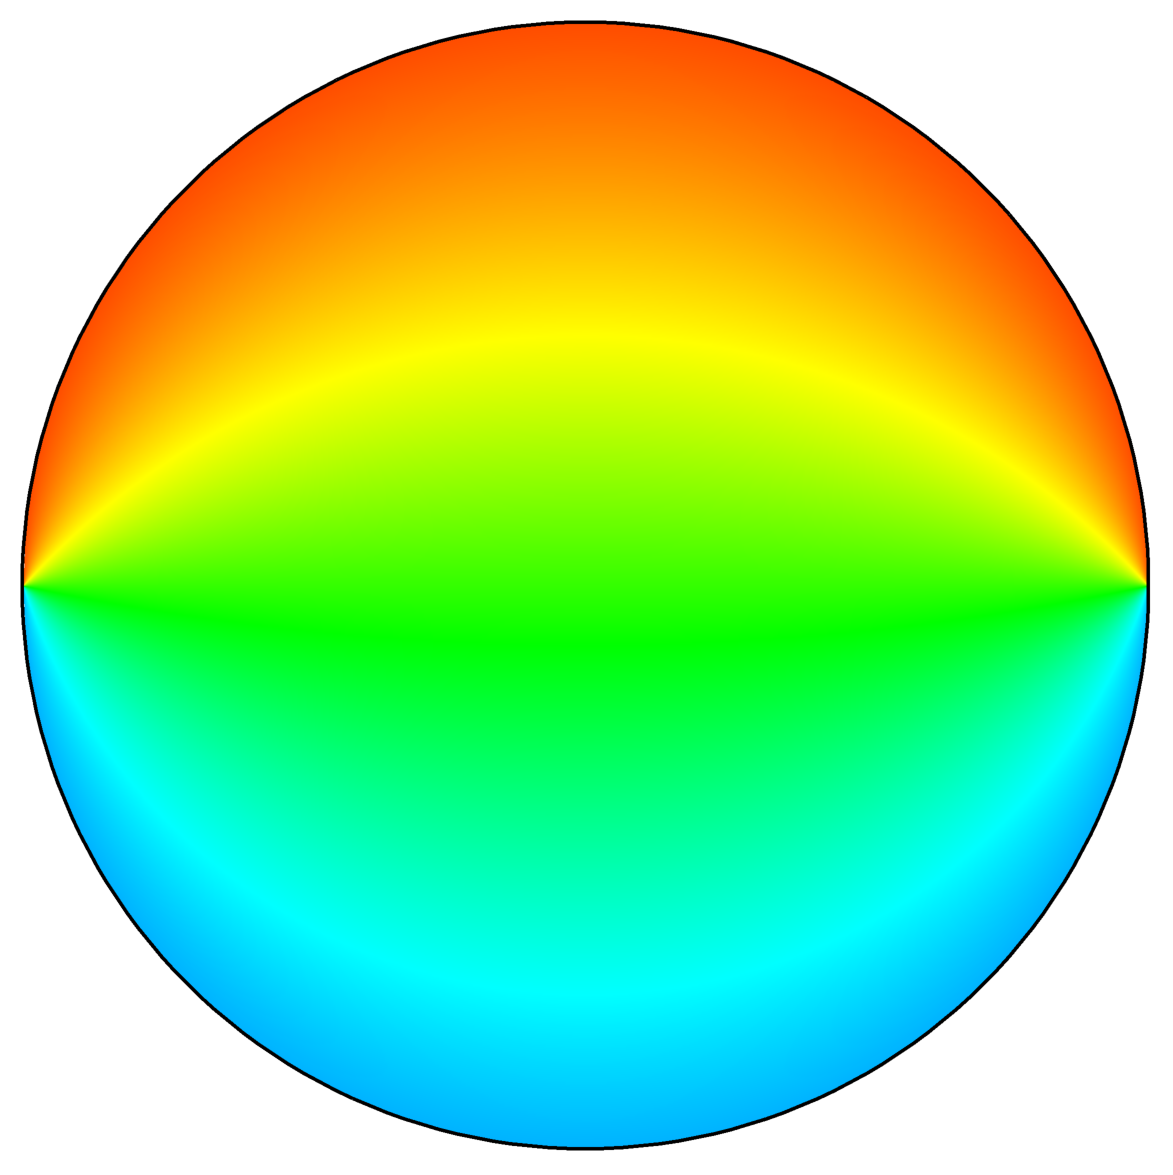
\includegraphics[scale=0.75]{potential.pdf}
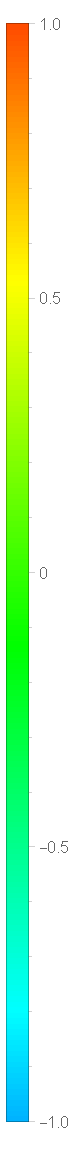
\includegraphics[scale=0.75]{potentscale.pdf}
\end{center}
\end{figure}

2. Similar to task 22.2.

3. If the current is $i$, then the rotating moment due to the Ampere force is
$$
  M=\frac12 BiR^2=J\dot{\omega}.
$$
Then the angular velocity depends on the total charge $q$ which passed through the system as
$$
  \omega=\frac{BqR^2}{2J}.
$$
Also, due to energy conservation,
$$
  qV=\frac{J\omega^2}{2}+\frac{Li^2}{2},
$$
which implies
$$
  \frac{L}{2}\left(\frac{2J}{BR^2}\right)^2 \dot{\omega}^2=\frac{2J}{BR^2} V\omega-\frac{J\omega^2}{2}.
$$
The solution of this equation is
$$
  \omega(t)=\frac{4V}{BR^2}\sin^2 \left(\frac{BR^2}{4J}\sqrt{\frac{J}{L}}t\right)=\frac{2V}{BR^2}\left(1-\cos\left(\frac{BR^2}{2J}\sqrt{\frac{J}{L}}t\right)\right).
$$
The corresponding expression for current is
$$
  i(t)=\frac{2V}{BR^2}\sqrt{\frac{J}{L}}\sin\left(\frac{BR^2}{2J}\sqrt{\frac{J}{L}}t\right).
$$

4. The bulk modulus $K$ is defined as
$$
  K=-V\frac{dP}{dV}.
$$
Integration gives
$$
  \ln\frac{V_0}{V}=\frac{p}{K},
$$
which yields
$$
  p=K\ln\frac{V_0}{V}=2\cdot 10^8 \text{ Pa}.
$$

\end{document} 